\documentclass{template/socthesis}

\usepackage{subcaption} 
\usepackage{amsmath} 
\usepackage{enumitem} 
\usepackage{hyperref} % reference
\usepackage{gensymb} % balíček symbolů
\usepackage{booktabs}

\usepackage[toc,page]{appendix}
\usepackage{color} % balíček pro obarvování textů
\usepackage{xcolor}  % zapne možnost používání barev, mj. pro \definecolor
\definecolor{mygreen}{RGB}{0,150,0} % nastavení barev odkazů 
\usepackage{listings} % balíček pro formátování zdrojových kódů 
\usepackage[author=,status=final]{fixme} % vkládání poznámek  
% dva módy (status): draft (poznámky se zobrazují v PDF) / final (poznámky se nezobrazují v PDF)
\usepackage{multirow}
\usepackage{hyperref} % pro vkládání odkazu

\lstset { %
    language=C++,
    backgroundcolor=\color{black!5}, % set backgroundcolor
    basicstyle=\footnotesize,% basic font setting
}

\addbibresource{text.bib} % soubor s bibliografií
\nocite{*}

\titlecz{Postav si svého druhého robota} % český název práce
\titleen{Build your second robot} % anglický název práce
\author{Tomáš Vavrinec} % jméno a příjmení autora
\field{7} % obor (pouze číslo, zbytek vysází šablona - číslo oboru viz http://www.soc.cz/obory-soc/)
\school{Střední průmyslová škola a~Vyšší odborná škola Brno, Sokolská, příspěvková organizace} % celý název školy
\mentor{Mgr. Miroslav Burda} % jméno a příjmení školitele
\mentorstatement{Mgr. Miroslava Burdy} % jméno a příjmení ve druhém pádě 

% Změňte, pokud se liší
%\region{Jihomoravský} % kraj
\placefooter{Brno 2020} % místo a rok

% hinty k používání balíčků hyperref, url, hyperlink a hypertarget
% \usepackage{hyperref} % balíček pro hypertextové odkazy
% \url{www.odkaz.cz}
% \href{http://www.odkaz.cz}{Text který bude jako odkaz}
% \hyperlink{label}{proklikávací_text} - odkaz na text 
% \hypertarget{label}{cíl_odkazu} - cíl odkazu 

\begin{document} % konec preambule dokumentu

\maketitle % vysází titulky

\makecopyrightstatement{V~Brně} % místo

% poděkování
\makethanks{Děkuji svému školiteli Mgr. Miroslavu Burdovi za obětavou pomoc, podnětné připomínky a~hlavně nekonečnou trpělivost, kterou mi během práce poskytoval.}

\pagestyle{empty}

\section*{Anotace}
% \color{mygreen}
% Anotace má za úkol stručně popsat cíle práce a velmi stručný úvod k tématu. 
% Většinou bývá použit první odstavec, nebo jiná část úvodu.
\color{black}

Robotika se stává čím dál tím významnějším oborem, což s sebou nese i potřebu vzdělávání v tomto oboru.
Při výuce robotiky jsou proto potřeba různé pomůcky na kterých se mohou žáci učit potřebné dovednosti. Jednou s takovýchto pomůcek 
by mohl být například SchoolBoard (viz práce Postav si svého prvního robota), ale pokročilejším studentům jiš tento hárdware nemusí
stačit. Proto jsem začal pracovat na novém systnému který má více možností.

\subsection*{Klíčová slova}

\color{black}

trezor, ESP32, ESP32 wrover, inteligentní ledky, WS2812, BMX055, LDC1614, LDC1314, open-source hardware

\newpage % pokud se anotace vleze na jednu stránku (což by měla), tento rádek zakomentuj

\vspace{20mm}

\section*{Annotation}
\color{black}

Robotics is becoming an increasingly important field, which brings with it the need for education in this field.
When teaching robotics, therefore, various aids are needed on which students can learn the necessary skills. Once with such aids
could be, for example, SchoolBoard (see the work Build Your First Robot), but for more advanced students this hardware may no 
longer need suffice. That's why I started working on a new system that has more options.

\subsection*{Keywords}
\color{black}
safe, ESP32, ESP32 wrover, smart leds, WS2812, BMX055, LDC1614, LDC1314, open-source hardware

\newpage
\pagestyle{plain}

\tableofcontents % vysází obsah

%%% Začátek práce
\setcounter{figure}{0}
\setcounter{table}{0}
\newpage

% zde můžeš s pomocí příkazu \input{cesta k souboru} vložit soubory; doporučuji každou větší kapitolu dát do samostatného souboru pro větší přehlednost


% Úvod práce

\chapter{Úvod}
%\addcontentsline{toc}{chapter}{Úvod}

Na konci července roku 2019 jsem dostal za úkol navrhnout výrobek pro děti na příměstský tábor pobočky DDM Helceletova Brno, \href{https://helceletka.cz/robotarna/}{Robotárny}.
Poža\-dav\-kem byla jednoduchá a levná konstrukce s elektronikou, kterou děti zvládnou sestavit za pár dní a ve zbytku času tábora si stihnou vyzkoušet základy programování 
s využitím tohoto výrobku. Z tohoto důvodu jsem začal vyvíjet elektronicky řízený trezor. Postup vývoje trezoru je popsán v kapitolách \ref{E-vyvoj} a~\ref{M-vyvoj}.

Z původní vize trezoru se ale rychle vyvinulo poměrně univerzální elektronické zařízení, kterému zůstala schopnost sloužit jako trezor.
Také využití trezoru se rozšířilo -- přibyly mu nové funkce a hlavním cílem už není pouze trezor  s dětmi stavět a programovat, 
ale také ho využívat jako herní prvek při táborových hrách. 
Trezor se tedy dá s dětmi jak stavět a učit s~jeho pomocí programování, tak ho využívat jako hotové zařízení při hrách pořádaných Robotárnou a dalšími subjekty.
Popis možností současné verze trezoru je v~kapitole \ref{E4}.

Dále přibyl požadavek na vývoj čistě mechanické varianty trezoru pro volnočasové aktivity, jednorázové akce nebo mladší účastníky táborů.
Mechanický trezor je z pochopitelných důvodů výrazně levnější než elektronický. Tím pádem se dá počítat s výrobou tohoto trezoru i na menších a levnějších akcích, ze kterých 
si účastníci trezor odnesou, což by v případě elektronické varianty znamenalo výrazně vyšší cenu i časovou náročnost.
Původně byla mechanická i elektronická verze vyvíjené tak, aby se mechanická verze dala jednoduše upravit na elektronickou, což popisuji v kapitole \ref{M1-vyvoj}.

Požadavky na elektroniku:
\begin{itemize}
    \item Zámek
    \item LED kruh
    \item Tlaková plocha
    \item Wifi
    \item Bluetooth
    \item Gyroskop
    \item Akcelerometr
    \item Magnetický kompas
    \item RTC (hodiny reálného času)
    \item Programátor s možností zákazu programování
    \item Barometr
    \item Nabíječka
    \item GPS
    \item GPRS
    \item IR komunikace
\end{itemize}

Z důvodů %todo
došlo oddělení obou verzí (viz kapitola %todo 
)
    % Trezor byl pro mě poněkud změnou oproti mé dřívějším práci, která se do té doby vždy točila kolem různých létajících nebo častěji jezdících robotů s velkým důrazem na orientaci v prostoru.
    % Trezor je oproti těmto vozítkům daleko statičtější, a protože se sám nepohybuje, má jeho vnímání prostoru jiné požadavky. Vozítka také vždy počítala s jistou univerzalitou senzoriky i~mechaniky,
    % zatímco trezor by měl být upravitelný jen po stránce softwaru. 

    % Další odlišností trezoru je menší konkurence, která je u různých robotických stavebnic poměrně veliká, jak si můžete přečíst 
    % v mé dřívější práci \href{https://github.com/TVavrinec/SOC-text/blob/master/SOČ.pdf}{Postav si svého prvního robota}.
    % Tato hračka/trezor/výrobek/zařízení je svým způsobem unikátní, jiné trezory (elektronizované, ve formě stavebnice pro děti/tábory) jsem zatím nikde nenašel. 

%todo popis, proč se oddělila mechanická a ele verze, původní záměr byl mít mecha verzi pro oba trezory stejnou  

%todo kapitola použití 

%todo zmínka o softwaru 

    % Na konci července roku 2019 jsem dostal za úkol navrhnout výrobek pro děti na příměstský tábor
    % pobočky DDM Helceletova Brno, Robotárny. 
    % Poža\-dav\-kem byla jednoduchá a levná konstrukce,
    % kterou děti zvládnou sestavit za pár dní a ve zbytku času tábora se jim ukážou základy programování
    % s~využitím tohoto výrobku. Proto, a také pro poněkud nižší věk účastníků, jsme se s vedoucím 
    % Robotárny, Jiřím Váchou, rozhodli jít cestou \uv{trezoru}. To byl rozdíl oproti našim běžným 
    % výrobkům, které většinou měly možnost pohybu, ale byly pro děti náročnější na výrobu
    % a pochopitelně i cena u nich šla nahoru.

%VARIANTA: 

%-- napsat cíl práce jako hotový, bez historie, vývoje a spol ... ???  

% Úvod práce má za cíl uvést:
% \begin{itemize}
%     \item cíl práce
%     \item jak ho chcete dosáhnout
%     \item popis tématu práce, musí být výstižný, ale stručný a poutavý
% \end{itemize}

\chapter*{vývoj}
\addcontentsline{toc}{chapter}{vývoj}

Na konci července roku 2019 jsem dostal za úkol navrhnout výrobek pro děti na příměstský tábor
pobočky D.D.M.Helceletova Brno, Robotárny. Požadavkem byla jednoduchá a levná konstrukce,
kterou děti zvládnou sestavit za pár dní a ve zbytku času tábora, se jim ukážou základy programování
s využitím tohoto výrobku. Proto, a i pro poněkud nižší věk účastníků, jsme se s vedoucím 
Robotárny, Jirkou Váchou, rozhodli jít cestou "trezoru". To byl rozdíl oproti našim běžným 
výrobkům, které většinou měly možnost pohybu, ale byly pro děti náročnější na výrobu
a pochopitelně i cena u nich šla nahoru.

\section*{první trezor}
\addcontentsline{toc}{section}{první trezor}

Dal jsem se tedy do kreslení trezoru, pochopitelně ne do nějaké nedobytné pevnosti, ale do malé
krabičky, na které se dají ukazovat principy elektronických zámků. Jelikož se mi na podobné
výrobky osvědčila jako materiál překližka, navrhoval jsem vše s úmyslem výroby z překližky 
za využití laseru. Konstrukce byla z velké části přizpůsobená dostupné elektronice, kterou 
jsem měl k dispozici, a která musela být stejně použita poněkud odlišně než jak byla zamýšlena.
Němel jsem totiž čas, a vlastně ani rozpočet, navrhovat a především vyrábět konkrétní elektroniku
pro výrobek, který se měl předložit dětem ani ne za týden. Použil jsem tedy starší univerzální 
desku ALKS (\href{https://github.com/RoboticsBrno/ArduinoLearningKitStarter}{Arduino Learnikg Kit Starter})
kterých jsem měl dostatečnou zásobu. Ovládací prvky, dvě tlačítka, dva potenciometry a tři
barevné ledky, tedy celý ALKS jsem umístil na horní stranu trezoru. ALKS má v původní variantě
tři tlačítka. Já jsem však jedno musel pomocí magnetu a jazýčkového magnetického konektoru použít
jako kontrolu, zda jsou dveře otevřeny či zavřeny. Jako zámek jsem pak použil obyčejné servo
SG90, které velice jednoduše zajelo svou páčkou do drážky ve dveřích, a tím jim zabránilo 
se otevřít. Celý systém pak napájela malá powerbanka, která se dala vyjmout a nabýt, 
a používala se i ve dvou dalších verzích. Tato konstrukce měla kvůli uspěchanému návrhu 
spoustu problémů. Většinou však šlo o problémy, které by nebylo těžké odstranit a nebylo
tedy třeba předělávat celý koncept návrhu. V těsném závěsu za touto elektronickou variantou,
jsem ale dostal požadavek i na čistě mechanickou verzi trezoru. To byl následně jeden z 
velkých důvodů velkých změn, a to i změny samotného konceptu zařízení.

\newpage
\section{První verze}
\label{M1-vyvoj}

\begin{wrapfigure}{R}[20mm]{0.4\textwidth}
    \centering
    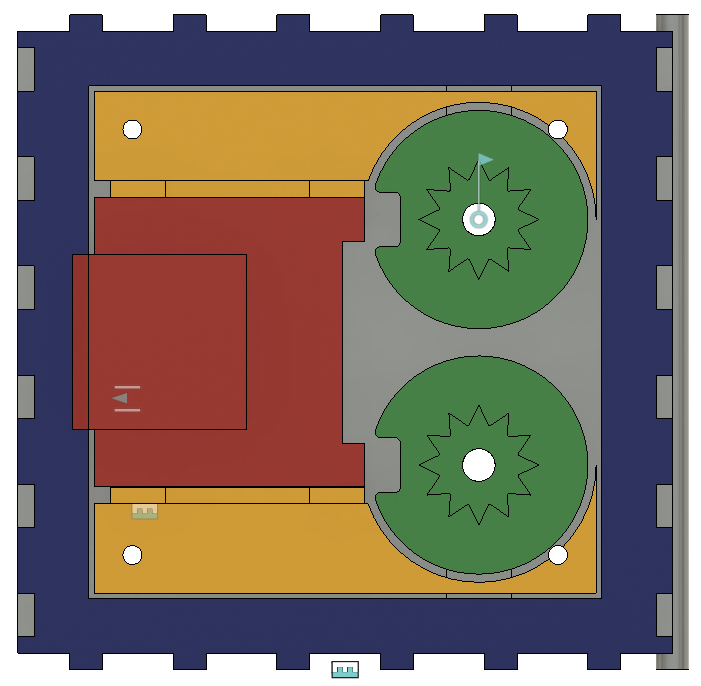
\includegraphics[width=0.4\textwidth]{kapitoly/obrazky/M1/mechanizmus.png}
    \caption{Zelená barva značí kódovací kola, červená západku, modrá pevnou část trezoru a žluté díly distanci \centering}
    \label{fig:M1-mechanizmus}
\end{wrapfigure}
První čistě mechanická varianta, označovaná jako M1, vznikla začátkem srpna 2019, brzy po první  elektronické variantě.
Měla stále poměrně klasický vzhled trezoru -- zamykatelná skříňka se dvěma  kódovacími koly, která ovládala možnost pohybu jednoduché západky.

Tato verze byla také určená jako základ pro plánovaný upgrade na další elektronickou
variantu. Na podobné vylepšení mělo stačit odstranění kódo\-va\-cích kol a přidělání elektronické části. Toto sice fungovalo obstojně, zároveň 
i~jako motivace, ale kvůli pozdější změně konceptu mechanizmu uzavírání trezoru\footnote{místo rotační západky mechanizmus bajonetu -- viz kapitola %todo
} tento nápad padl.

Tato varianta se také ukázala jako nevhodná\footnote{kvůli přílišné náročnosti na přesnost sesazení} pro stavbu s malými dětmi, 
pro které byla určena jakožto předstupeň k variantě elektronické (která vyžaduje i~znalosti programování nebo alespoň ochotu se jej  učit).

\newpage
\section{Druhá verze}
\label{E2-vyvoj}
Druhá verze trezoru už byla vybavená signalizačním kruhem o dvanácti LED kolem uprostřed dveří
umístěného enkodéru. Jako základ trezoru jsem použil první mechanický trezor \ref{M1-vyvoj},
a doplnil jej o servo, řídící elektroniku a již zmíněný kruh LED a~enkodér.
%Vzhledem k tomu, že se jednalo jen o hrubý prototyp, neměl specializovanou desku~a elektroniku  tedy tvořila jen změť kabelů 
% a kousek univerzální desky, takže nemám elektronickou variantu tohoto zapojení. % [schéma jsem kreslil jen na tabuli a to asi rok 
% zpátky, takže když bych došel k závěru že je potřeba, tak se dá udělat, ale je to práce navíc a nepovažoval bych to za podstatné]

Trezor měl pro komunikaci s uživatelem tedy kruh o dvanácti LED a~jeden vstupní prvek -- enkodér s tlačítkem.
Ovládání bylo od výbavy trezoru odvozené a trezor se zmáčknutím tlačítka na enkodéru zapnul a tlačítko pak dál sloužilo jako potvrzování výběru.
Uživatel tak mohl pomocí enkodéru vybírat jedinou rozsvícenou ledku a stiskem potvrdit. 

Vstupní kód tedy mohl vypadat 
například jako čas a uživatel ho zadal na kruhu odvozeném od ručičkových hodin, proto právě dvanáct LED.
Konkrétní ovládání je pochopitelně závislé na nahraném programu a mohlo by se tedy jednoduše změnit do libovolné podoby --
to, co popisuji, je jen konkrétní možnost, kterou jsem použil. 

Vzhled tohoto trezoru na obrázku \obr{fig:E2-render}

\newpage
\section{Druhá verze}

Druhá mechanická varianta má oproti první verzi daleko vetší počet možných kombinací.
Ovládá se pěti koly. Čtyři z nich nastavují heslo a páté otáčí s~rotační západkou, která drží dveře na svém místě.

Tato varianta taky přichází s možností dveře úplně oddělit od skříně trezoru. To by při využití jako trezor, který
má za úkol jen ochraňovat svůj obsah, sice nepřinášelo žádný velký užitek, ale při mém využití, spíše jako herní 
prvek než trezor, to může být užitečné.

\begin{figure}[htbp]
    \centering
    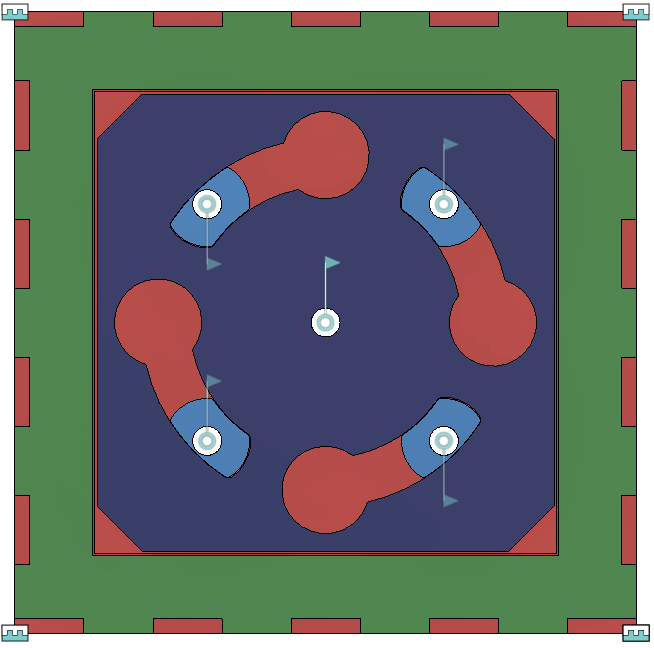
\includegraphics[width=150pt]{kapitoly/obrazky/M2/mechanizmus_odemcen.png}
    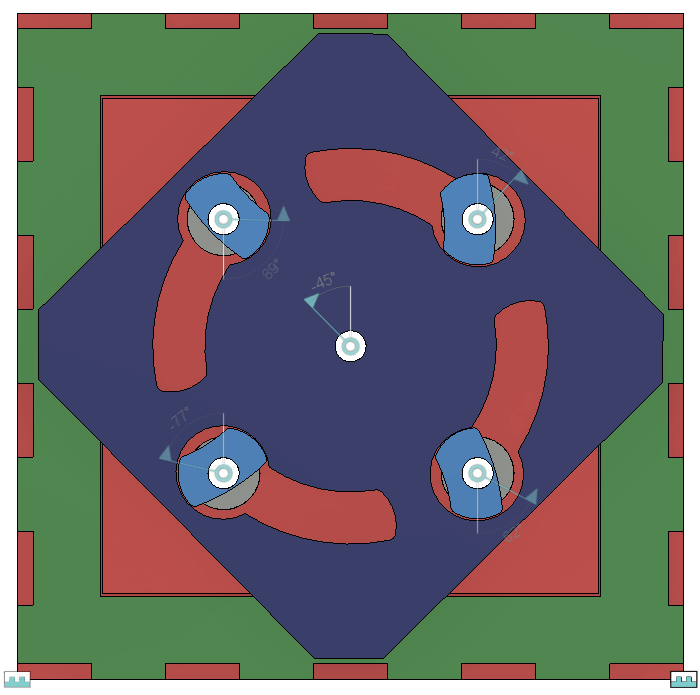
\includegraphics[width=150pt]{kapitoly/obrazky/M2/mechanizmus_zamceno.png}
    \caption{zamykací mechanizmus varianty M2}
    \label{fig:M2-mechanizmus}
\end{figure}

\begin{figure}[htbp]
    \centering
    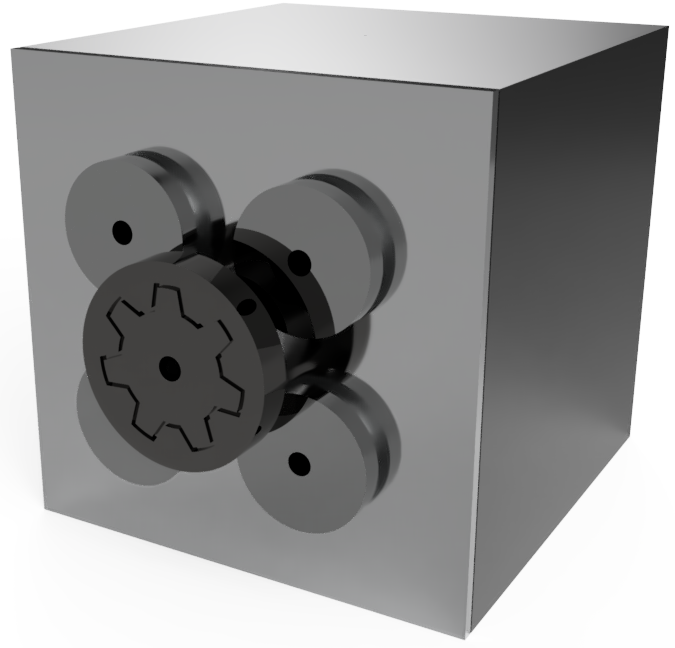
\includegraphics[width=\textwidth]{kapitoly/obrazky/M2/predni_render.PNG}
    \caption{render varianty M2}
    \label{fig:M1.0}
\end{figure}


\newpage
\section*{Třetí elektronická varianta}
\addcontentsline{toc}{section}{Třetí elektronická varianta}

Třetí verze elektronické varianty do značné míry vycházela z předchozí, druhé verze, a dále na ní stavěla. Asi nejzjevnější změna bylo navýšení počtu 
ledek z dvanácti, jakožto hodiny, na šedesát jakožto minuty, což pochopitelně znamenalo i zvětšení kruhu. Na desku se ale přidaly i nové funkcionality,
a to gyroskop, pro možnost znalosti náklonu zařízení, akcelerometr, pro znalost směru a velikosti zrychlování, magnetický kompas, pro určení světových
stran, RTC (Real Time Clock, hodiny reálného času), pro znalost přesného času a také GPS pro možnost určení svojí polohy.
Také jsem použil, po vzoru mechanické varianty, rotační západku, což znamenalo, že na stejný trezor se daly použít jak mechanické tak 
elektronické dveře.

Tato verze měla dvě podverze, které se lišily motorem.
\begin{figure}[htbp]
    \centering
    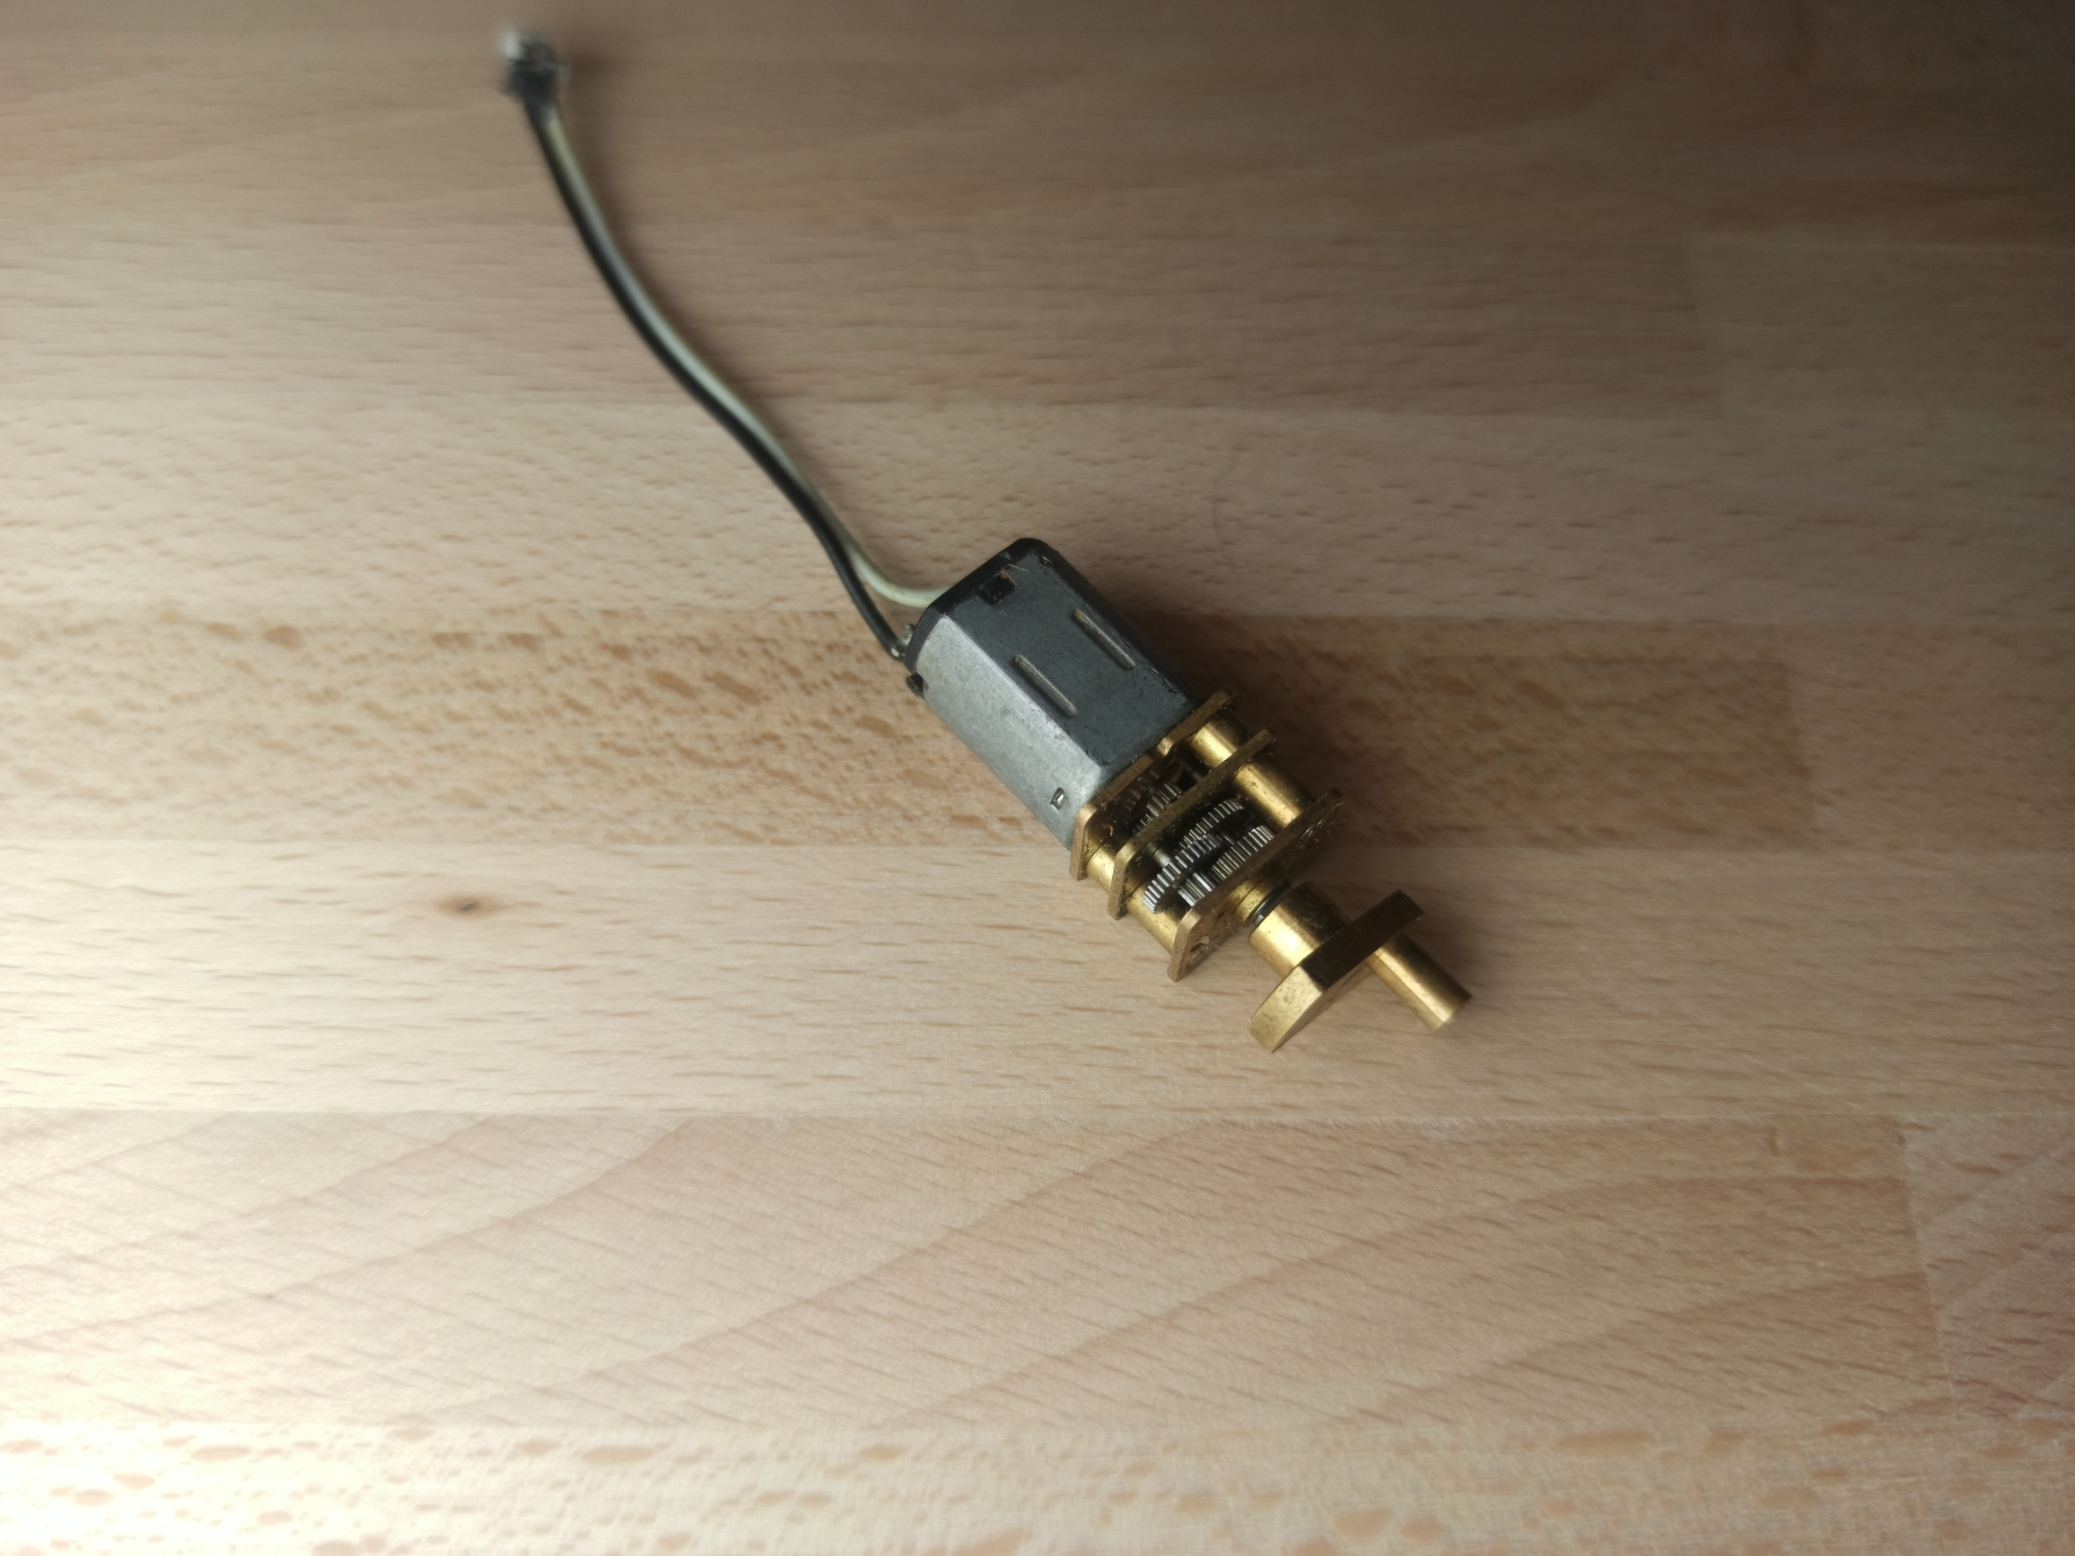
\includegraphics[width=160]{kapitoly/obrazky/E3/motory/hodinovyStrojek.jpg}
    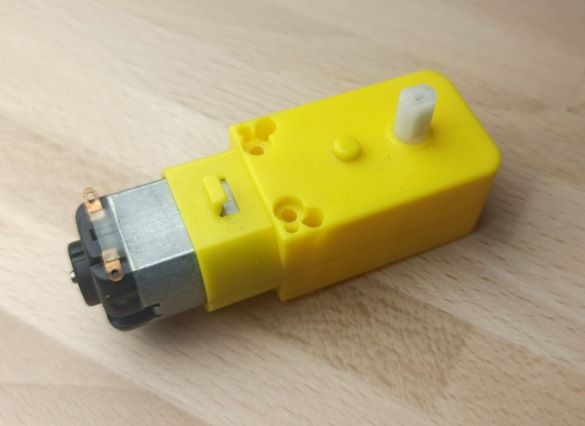
\includegraphics[width=160]{kapitoly/obrazky/E3/motory/zluty_motor.jpg}
    \label{fig:M1}
\end{figure}

\begin{figure}[htbp]
    \centering
    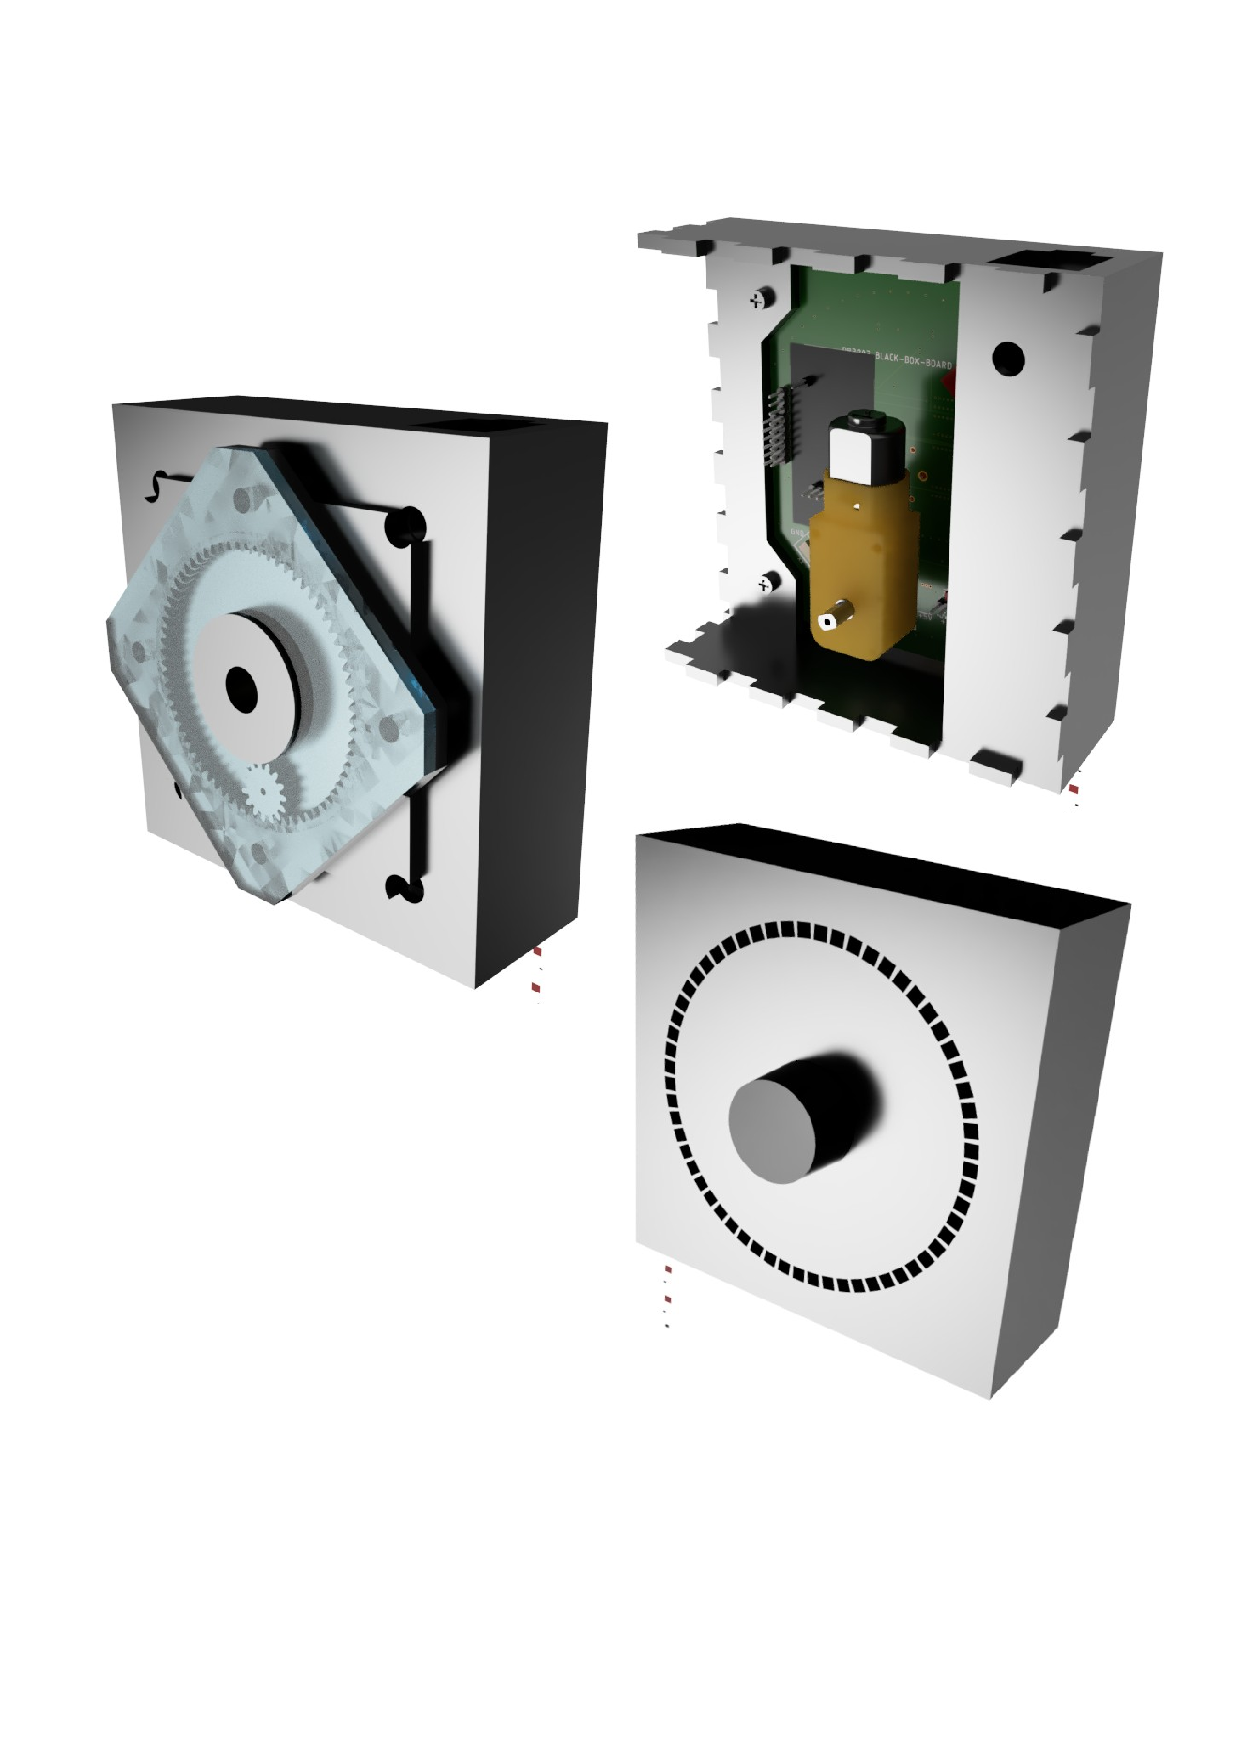
\includegraphics[width=\textwidth]{kapitoly/obrazky/E3/rendery.pdf}
    \label{fig:M1}
\end{figure}

Přes velké množství funkcí jsem, kvůli několika věcem ale opět koncept přepracoval. Hlavním důvodem změn bylo náročné uložení rotační západky, 
které vyžadovalo ozubený věnec a několik dalších tisknutých dílů.

\newpage
\section{Čtvrtá verze}
\label{E4-vivoj}

\subsection*{Rozšíření elektroniky}

Čtvrtá verze byla co se elektroniky týče přímým pokračováním předchozí verze (viz kapitola \ref{E3-vyvoj}), kterou dále rozšiřuje.

Trezor získal oproti minulé verzi schopnost komunikace pomocí IR z důvodu identifikace růz\-ných dveří, dále získal magnetický enkodér, pro možnost snaz\-ší\-ho ovládání
motoru zámku. 
Další inovací byl programovací systém s~USB-C, na místo USB-micro jako dřív. Nový programátor má možnost úplně si odpojit napáje\-ní, a~to~v~rámci šetření 
energie, když trezor programátor nevyužívá. 
Zároveň umožňuje zákaz přeprogramování.

Podstatnou změnou také bylo rozdělení elektroniky do dvou různých desek, protože na jedné by nebyl dostatek místa. Jedna deska \obr{fig:E4-sch_next-board}, \obr{fig:E4-LedDeska}
tak obsahuje kruh LED \parencite{WS2812} a čip LDC1614 \parencite{LDC1614} nebo LDC1314 se čtyřmi cívkami, které měří vzdálenost tlakové desky. Na druhé desce
je vše ostatní, tedy procesor \parencite{ESP32}, akcelerometr a
gyroskop \parencite{bmx055}, \parencite{mpu6050}, magnetický kompas \parencite{bmx055}, \parencite{qmc5883}, RTC\footnote{Real Time Clock, hodiny reálného času} \parencite{m41t62}, 
barometr \parencite{spl06}, IR vysílač \parencite{ir19-21c/tr8} a přijímač \parencite{irm-h936}, magnetický enkodér \parencite{mh253}, \parencite{ss360nt}, programátor \parencite{cp2102},
řešení napájení, řízení motoru a nabíječka \parencite{se9017}. 

\subsection*{Princip zamykání}

Na trezoru se dále změnily princip zamykání a ovládání. 

Důvodem změn bylo náročné uložení rotační západky, 
které vyžadovalo ozubený věnec a několik dalších tisknutých dílů.
Z tohoto důvodu také již není možné použít tělo mechanického trezoru pro elektronickou variantu.

Zamykání je založeno na mechanizmu bajonetu a zamčení je zajištěno západ\-kou, která zabraňuje zpětnému otočení.
Západka je ovládána motorem, který otáčí magnetem a přitahuje nebo odpuzuje magnet na západce. Důvodem pro magnetické ovládání
byla možnost západku ovládat i přes pevnou stěnu, a~také pružné spojení, které takto vznikne, takže se trezor například dá zavřít, i~když
je už zamčen (když například dveře nejsou dovřeny).

\begin{figure}[htbp]
    \centering
    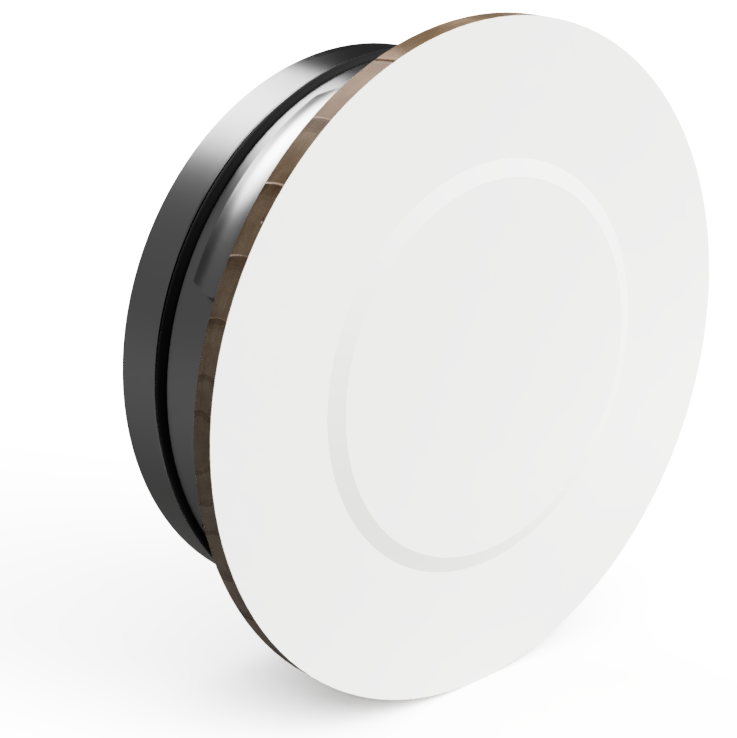
\includegraphics[width=170pt]{kapitoly/obrazky/E4/predni_render.png}
    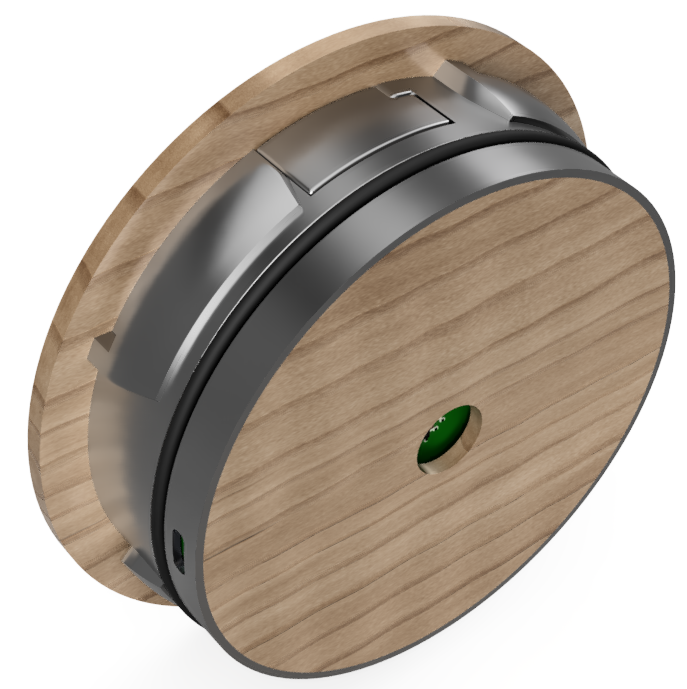
\includegraphics[width=170pt]{kapitoly/obrazky/E4/zadni_render.png}
    \caption{Rendery dveří trezoru E4 -- vlevo přední pohled, vpravo zadní pohled \centering}
    \label{fig:E4-render}
\end{figure}

\subsection*{Ovládání}
Předchozí varianty měly jako hlavní ovládací prvek enkodér s tlačítkem, ten jsem v nynější variantě odstranil, aby přední stěna neměla tak velký 
výstupek. Proto jsem tento prvek nahradil indukční tlakovou deskou \ref{E4-tlakovka}, která vyplnila vnitřek kruhu ledek \ref{WS2812}. 
Zbytek ovládání víceméně přetrval, jen kvůli nedostatku času a~pandemií způsobenému nedostatku součástek, trezor přišel o GPS.\footnote{Deska má ale stále možnost připojení GPS pomocí konektoru.}
Na druhou stranu ale získal barometr s rozlišením schopným detekovat změnu výšky o půl metru.

\subsection*{Napájení}
Předchozím verzím sloužila jako napájení powerbanka. Ta však kladla poměrné velké omezení, dokázala poskytnout proud pouze jednoho ampéru, a proto 
jsem jí nahradil vlastním zdrojem, dvěma bateriemi 18650. 
To samozřejmě znamenalo nutnost vlastního řešení stabilizace napětí, díky čemuž trezor dostal stepup FP6276 \parencite{fp6276a}, \obr{fig:E4-step-up}, 
který spíná napětí z 3,5~V až 4,2~V na 5~V, a původně stepdown, později lineární stabilizátor \obr{fig:E4-stabilizator}, který poskytuje 3,3~V. 

Trezor také dostal vlastní nabíječku, aby pro nabíjení baterií stačilo připojit kabel, stejně jako třeba u mobilu.



\chapter*{Mechanická varianta}
\addcontentsline{toc}{chapter}{Mechanická varianta}


\chapter*{Elektronicka varianta}
\addcontentsline{toc}{chapter}{Elektronicka varianta}

\section{Přehled}

Dnešní verze elektronického trezoru se zamyká pomocí mechanizmu bajonetu a magneticky řízené zpětné západky. 

Elektronika je vybavena čipem ESP32 \parencite{ESP32}, \parencite{ESP32-WROVER-B},
který obsahuje dva procesory Xtensa LX6, WiFi a bluetooth. Dále je trezor vybaven čipem BMX055 \parencite{bmx055} nebo dvojicí čipů MPU6050 \parencite{mpu6050} 
a QMC5883 \parencite{qmc5883} které poskytují 
gyroskop, akcelerometr a magnetický kompas. Dále je zde SPL06 \parencite{spl06}, barometr s rozlišením 0,06~hPa, což umožňuje rozeznat změnu nadmořské výšky 
o polovinu metru. Další systém trezoru je možnost IR komunikace, která je zde pro možnost jednoznačné identifikace dveří, ale pochopitelně může 
sloužit i pro jiný účel. Deska je také vybavena RTC \footnote{Real Time Clock, hodiny reálného času} a má vlastní programátor pro usnadnění programování. Vedle ESP32 je zde asi 
nejvýznamnějším čipem LDC1614 \parencite{LDC1614}, případně LDC1314, který umožňuje funkci tlakové plochy (viz kapitoly \ref{E4-tlakovka} \ref{E4-mech_tlakovky}).

%todo doplnit popis a využití a možnosti tlakové desky 

\begin{table}[h]
    \centering
    \resizebox{\textwidth}{!}{%
    \begin{tabular}{@{}lll@{}}                                                                                 \\ \midrule
    \textbf{ESP32}              & dva procesory Xtensa LX6, WiFi a bluetooth    &                                                                           \\
    \textbf{BMX055}             & gyroskop, akcelerometr, magnetický kompas     & možno nahradit dvojicí čipů MPU6050 a QMC5883                             \\
    \textbf{SPL06}              & barometr                                      & rozlišení až 0,06hPa což umožňuje rozeznat změnu nadmořské výšky o 0,5m   \\
    \textbf{IRM-H936 a IR led}  & IR komunikace                                 &                                                                           \\
    \textbf{LDC1614}            & snímání tlakové desky                         & počítá se s možnou záměnou za LDC1314                                     \\
    \textbf{CP2102}             & programátor                                   & s hardwarově zajištěným odpojováním napájení, pokud není využíván          \\ \bottomrule
    \end{tabular}%
    }
    \caption{Shrnutí elektronického vybavení}
    \label{tab:COMPARATION}
\end{table}

\newpage
\section{Mechanika tlakové desky}
\label{E4-mech_tlakovky}

Indukčně snímaná tlaková deska funguje díky čtyřem cívkám na desce ploš\-ných spojů, které mění svojí indukčnost podle vzdálenosti snímané desky, terčíku.
Z tohoto důvodu se terčík při používání naklání, čímž zároveň mění svojí vzdálenost od jednotlivých cívek. Z toho také plyne nutnost uložit terčík
částečně volně. Terčík je proto od snímací desky oddělen pružnou vložkou, která je zároveň předepnuta pomocí nažehlovací fólie, která kryje přední 
stranu dveří a spojuje terčík s čelní krycí deskou. Díky nažehlovací fólii je také přední část dveří voděodolná.

\begin{figure}[h]
    \centering
    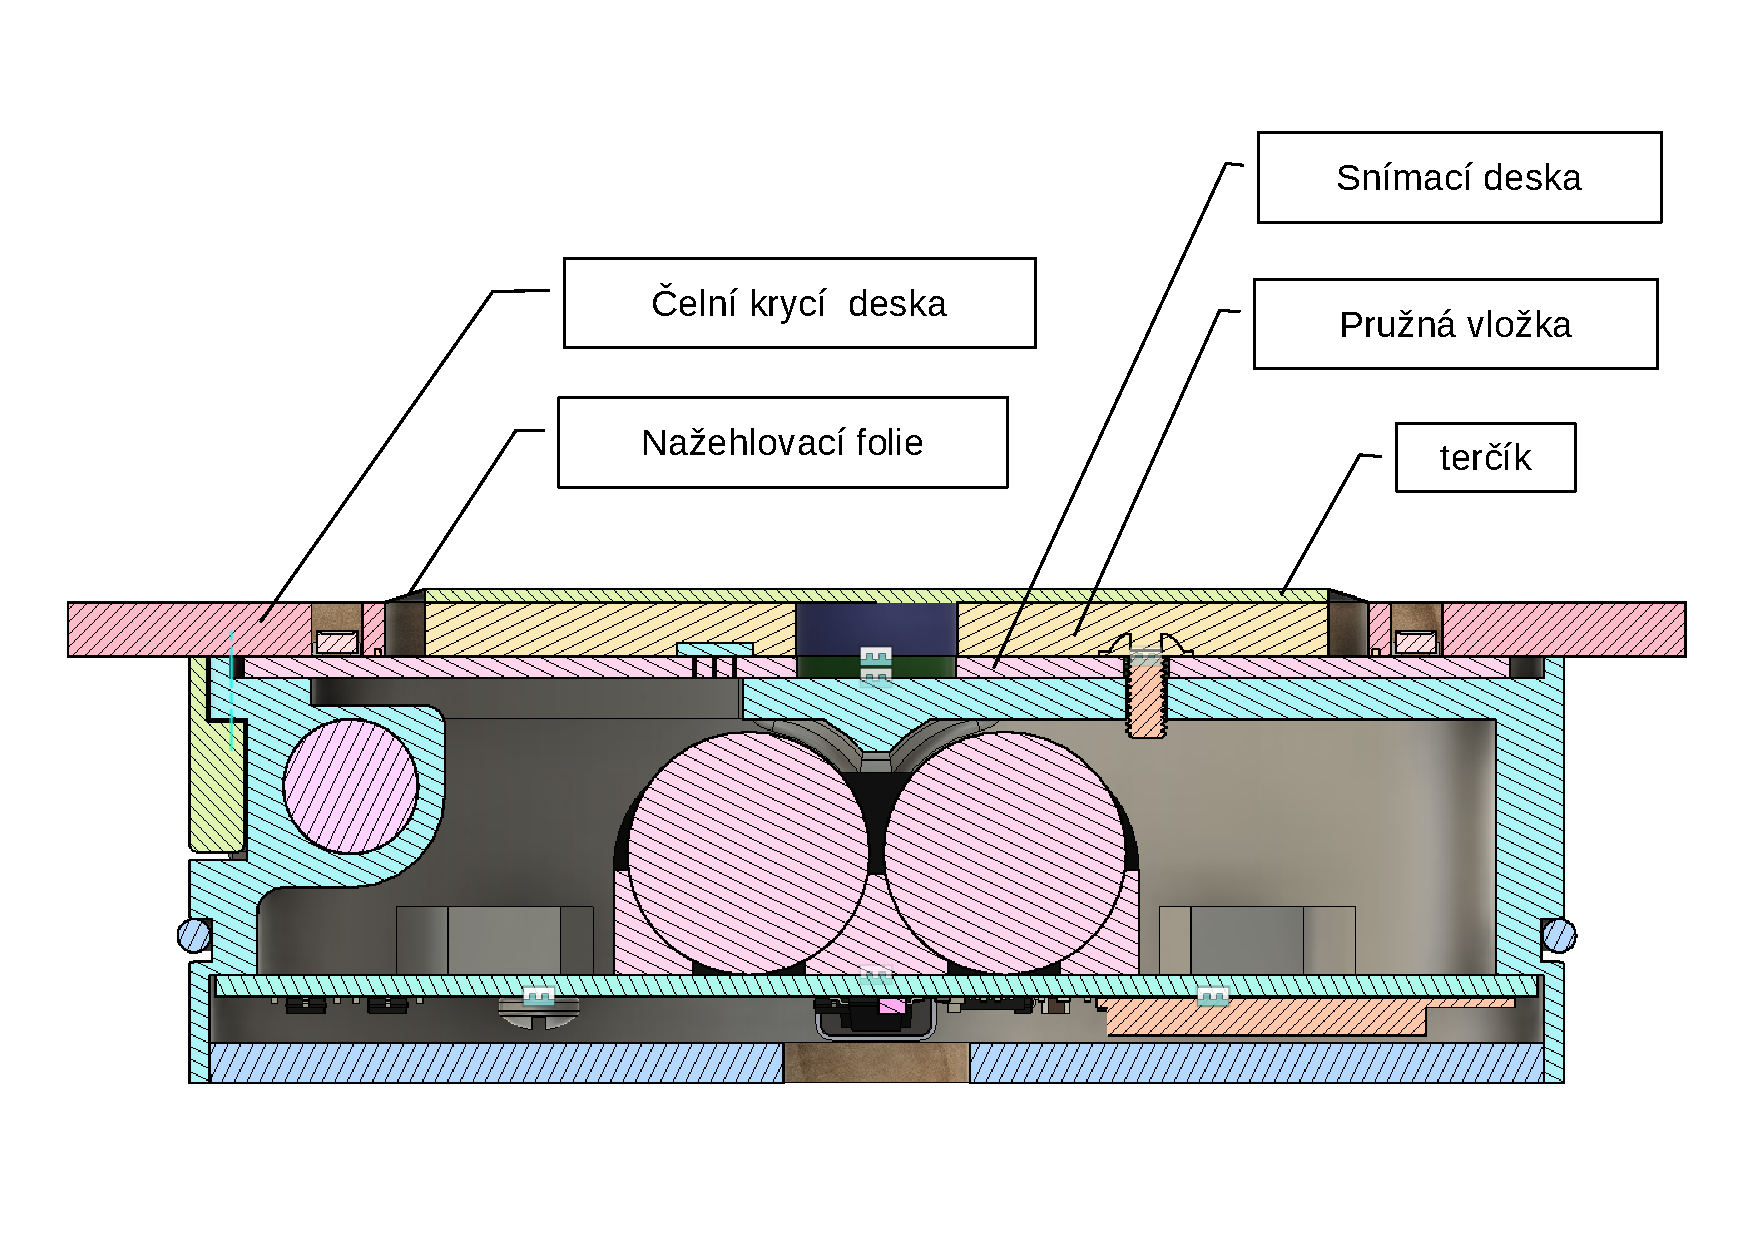
\includegraphics[width=\textwidth]{kapitoly/obrazky/E4/machanika_tlakove_desky/rez_po_ose.pdf}
    \caption{Řez varianty E4}
    \label{fig:E4-rez}
\end{figure}

\newpage

Díky zkušenostem z jiného podobného projektu jsem zjistil, že ovládací prvek by měl být co možná největší. 
Zároveň by měl odolat i poměrně silným ranám, které děti v zápalu hry zařízení uštědřují.
Tlaková deska tedy počítá s možností působení síly o velikosti až 500~N, což samozřejmě zároveň znamená, že tělo dveří tomuto zatížení musí odolat.
Vzhledem k tomu, že nemám možnost vyrobit tělo z kovu a jsem odkázán na 3D tisk a laserovou řezačku, a zároveň chci mít dveře co možná nejmenší,
musel jsem napočítat kritické části těla tak, aby odolaly a zároveň nebyly příliš mohutné. Z tohoto důvodu jsem v programu Fusion 360, ve kterém jsem trezor vyvíjel,
dělal simulaci, kterou k práci přikládám na obrázcích \obr{fig:E4-simulace_tela} a \obr{fig:E4-simulace_tlakovky}.

Jako materiál těla jsem v první fázi zvolil standardní fotopolymer pro tiskárny typu SLA, s pevností v tahu 46 až 67 MPa.
V budoucnu bych ale chtěl tělo odlévat z nějakého houževnatého polyuretanu, aby se zlevnila výroba a zároveň stoupla odolnost.



% Zaver prace
\chapter*{Závěr}
V závěru by mělo být:
\begin{itemize}
    \item Rekapitulace cíle práce
    \item Dosáhnul jsem jej? Ano, nebo ne?
    \item Zhodnocení průběhu práce
    \item Co mi práce dala?
\end{itemize}

\newpage
\newpage

\appendix
\addcontentsline{toc}{chapter}{Přílohy}

% Prilohy
% \chapter{Obrazové přílohy}

\begin{figure}[h]
    \centering
    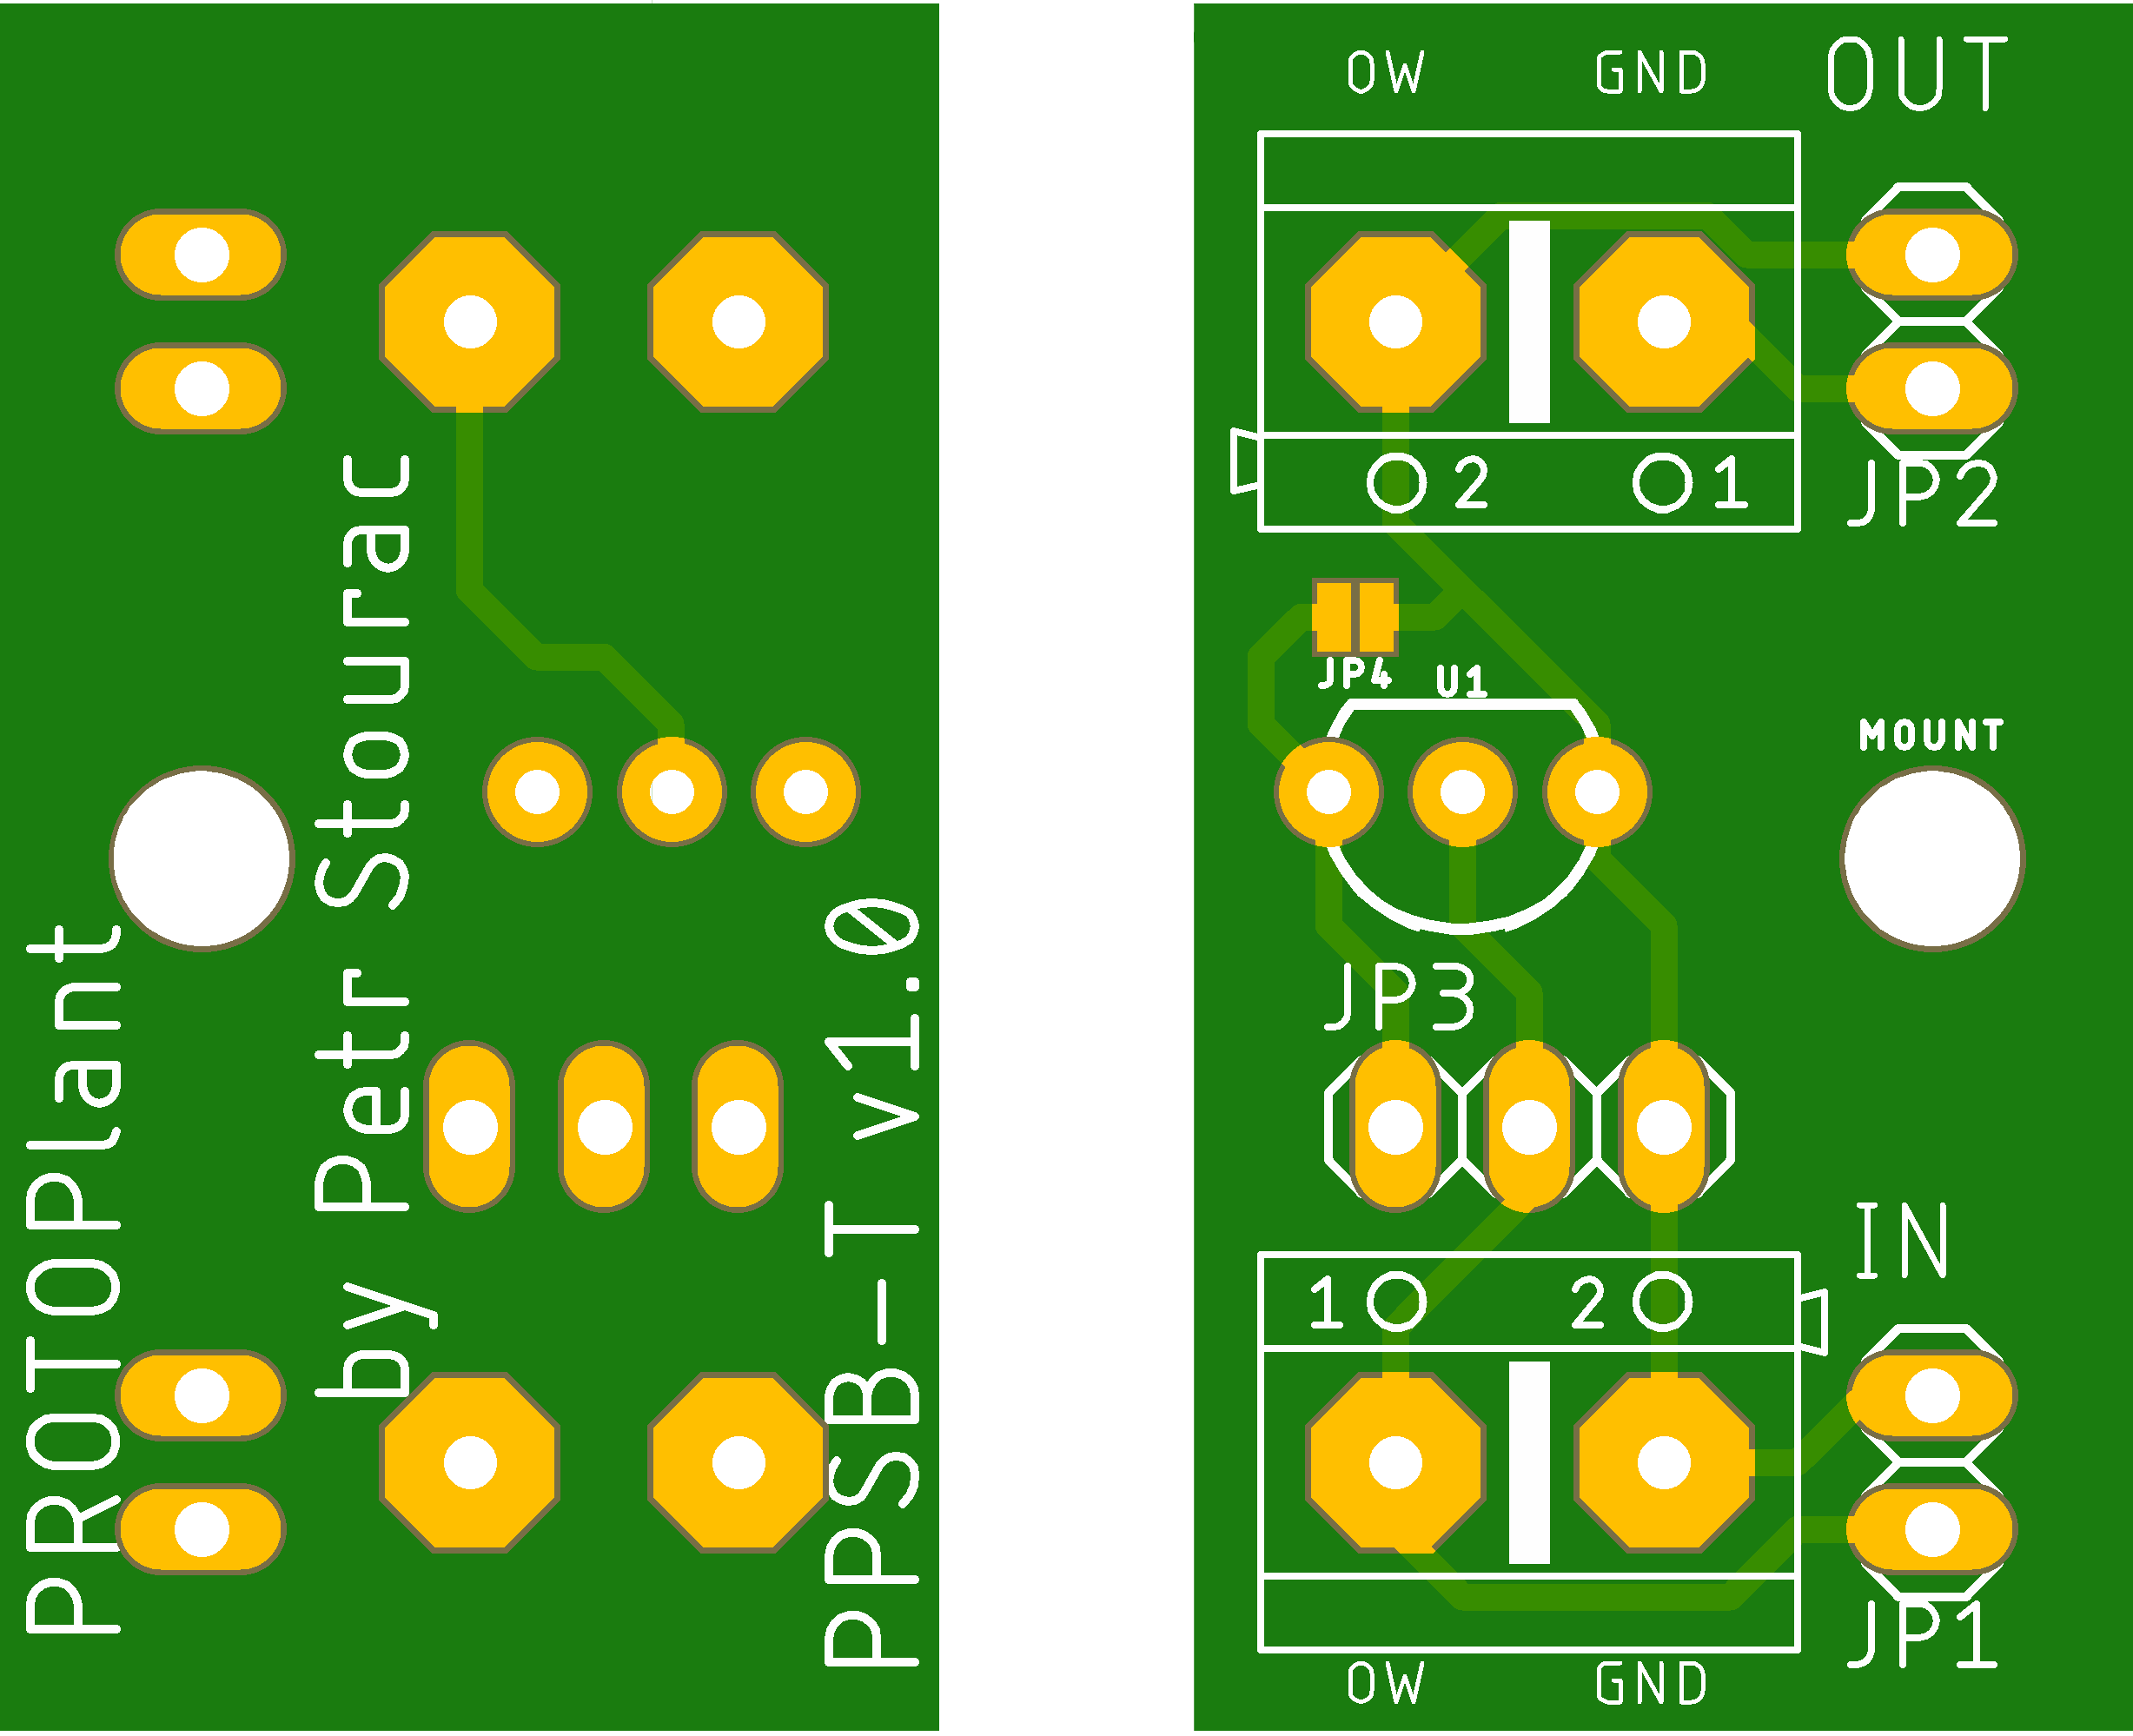
\includegraphics[width=0.85\textwidth]{img/HARDWARE/PPSB-T_BOTH.png}
    \caption{Vizualizace PPSB-T (horní strana vpravo, dolní vlevo).}
    \label{fig:PPSB-T_VISUAL}
\end{figure}

\begin{figure}[h]
    \centering
    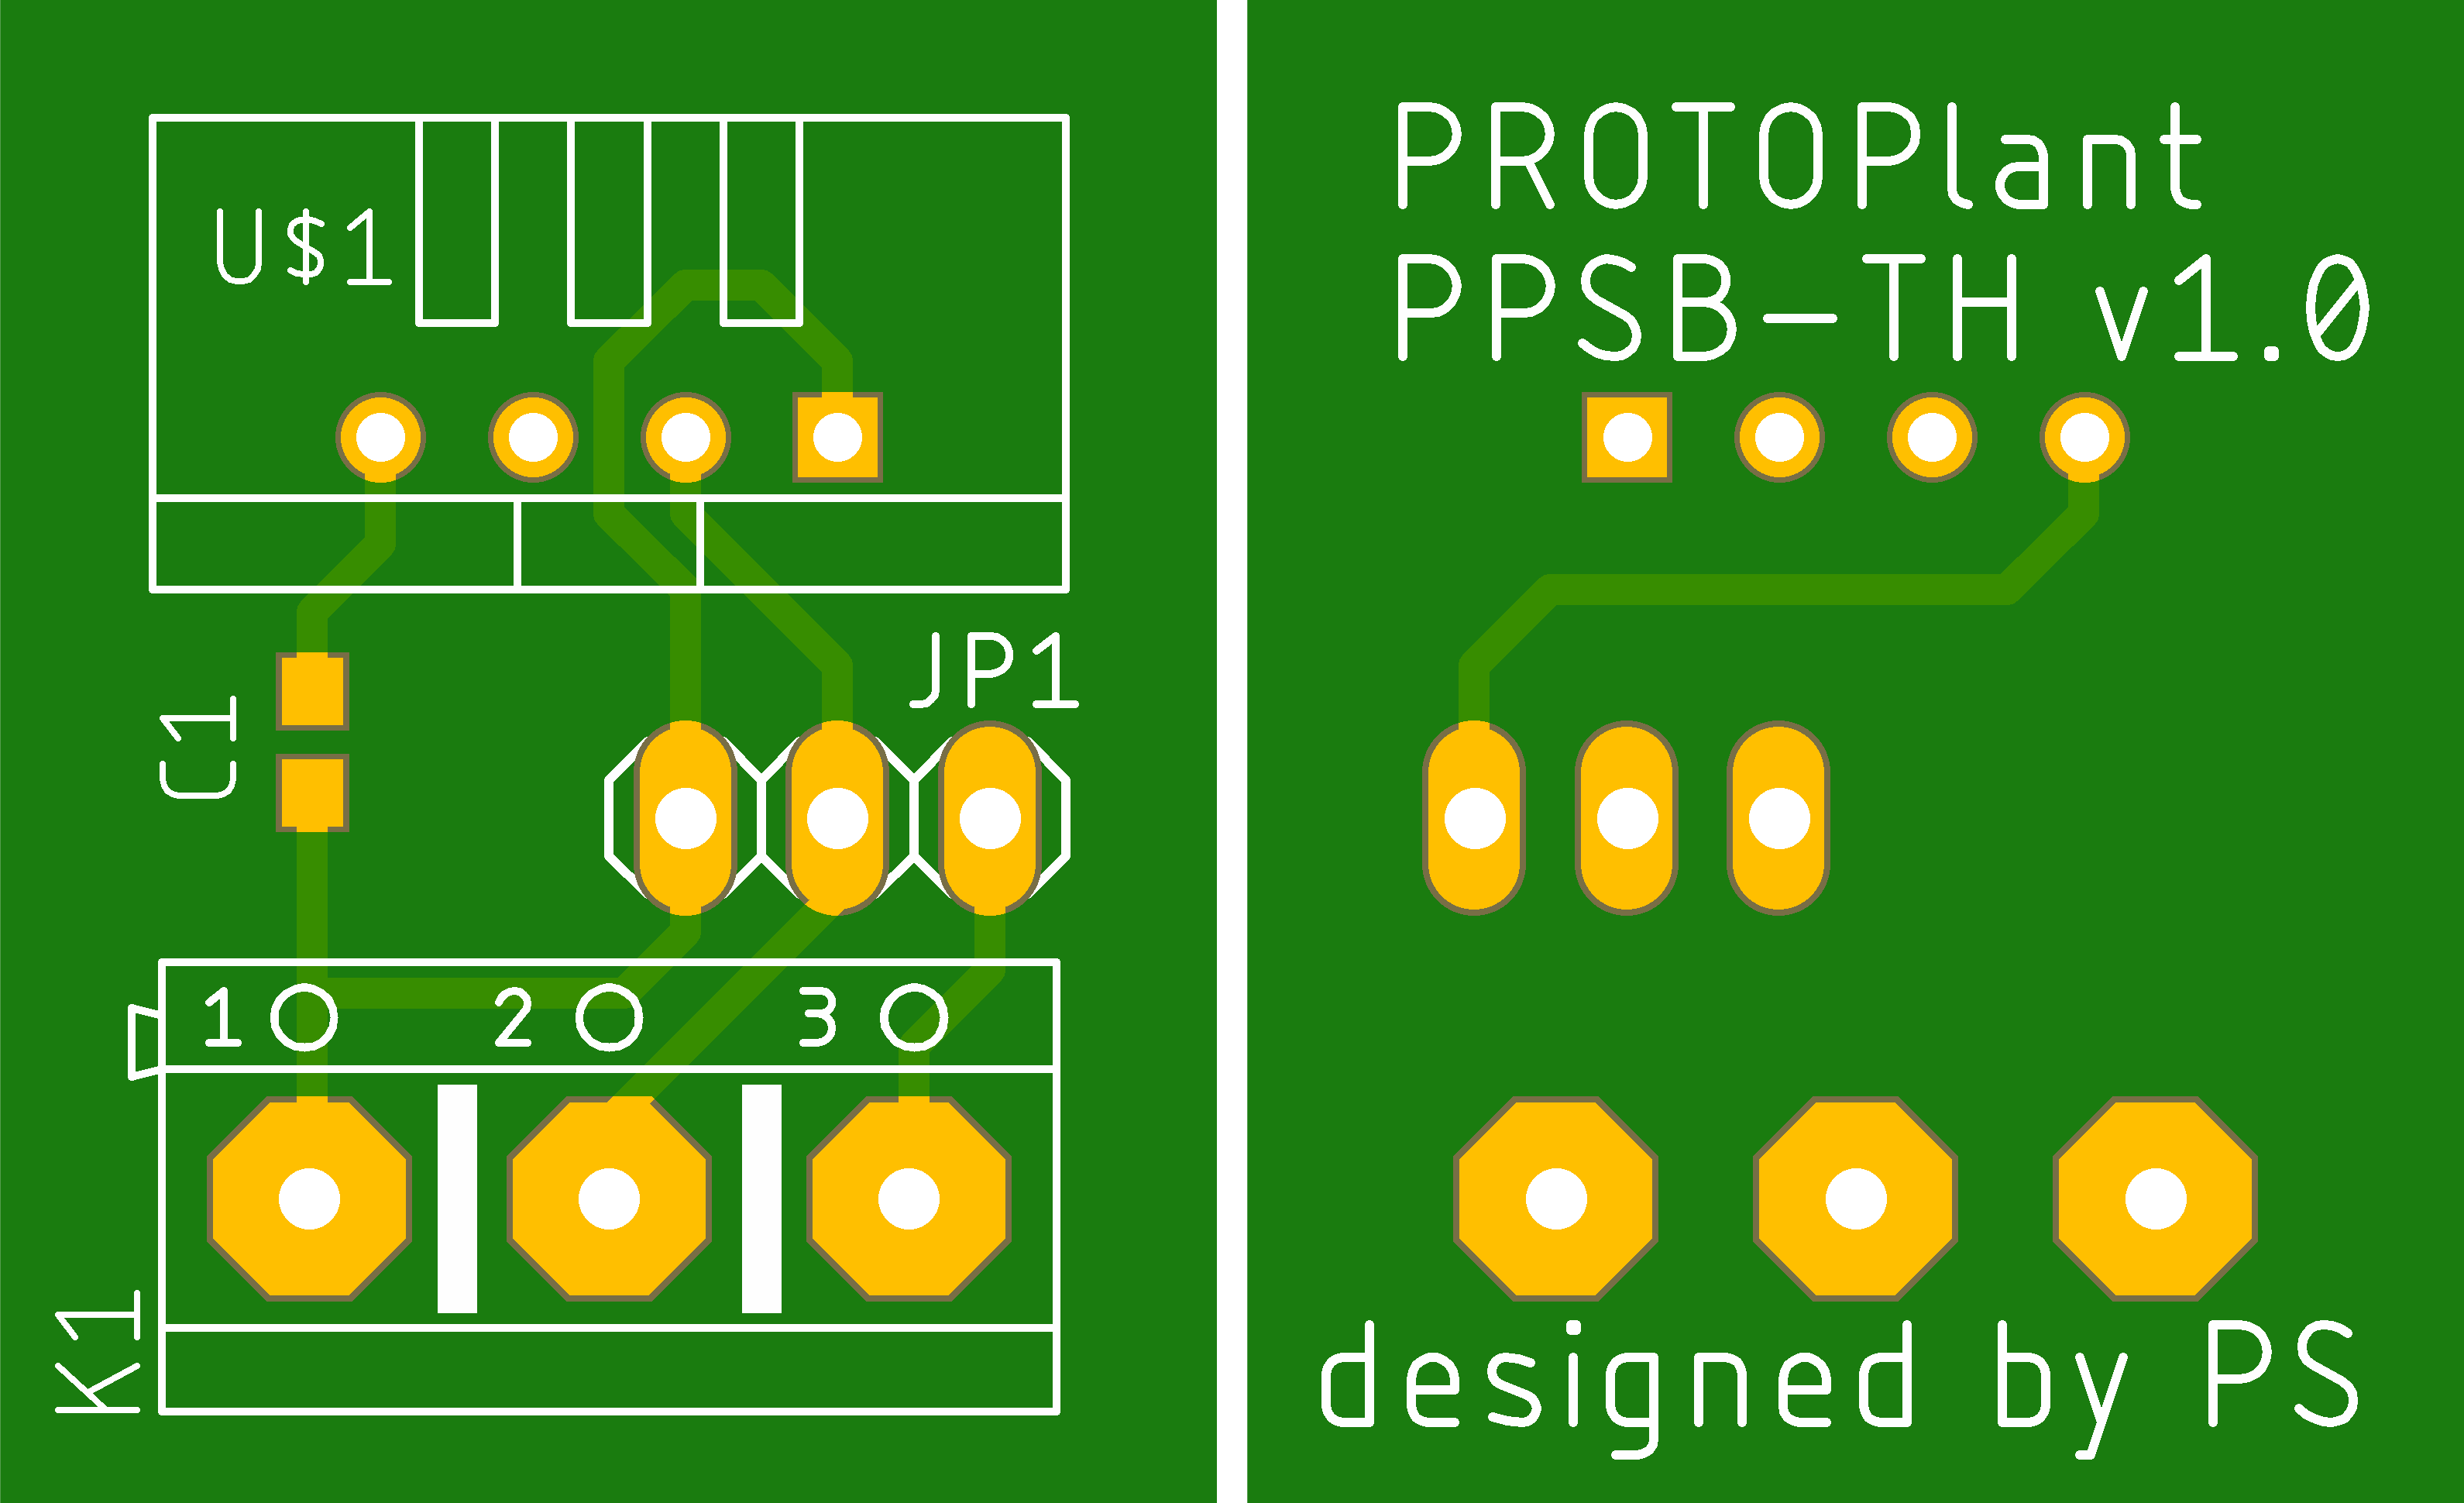
\includegraphics[width=0.85\textwidth]{img/HARDWARE/PPSB-TH_BOTH.png}
    \caption{Vizualizace desky PPSB-TH (horní strana vlevo, dolní vpravo).}
    \label{fig:PPSB-TH_VISUAL}
\end{figure}

\begin{figure}[htbp]
    \centering
    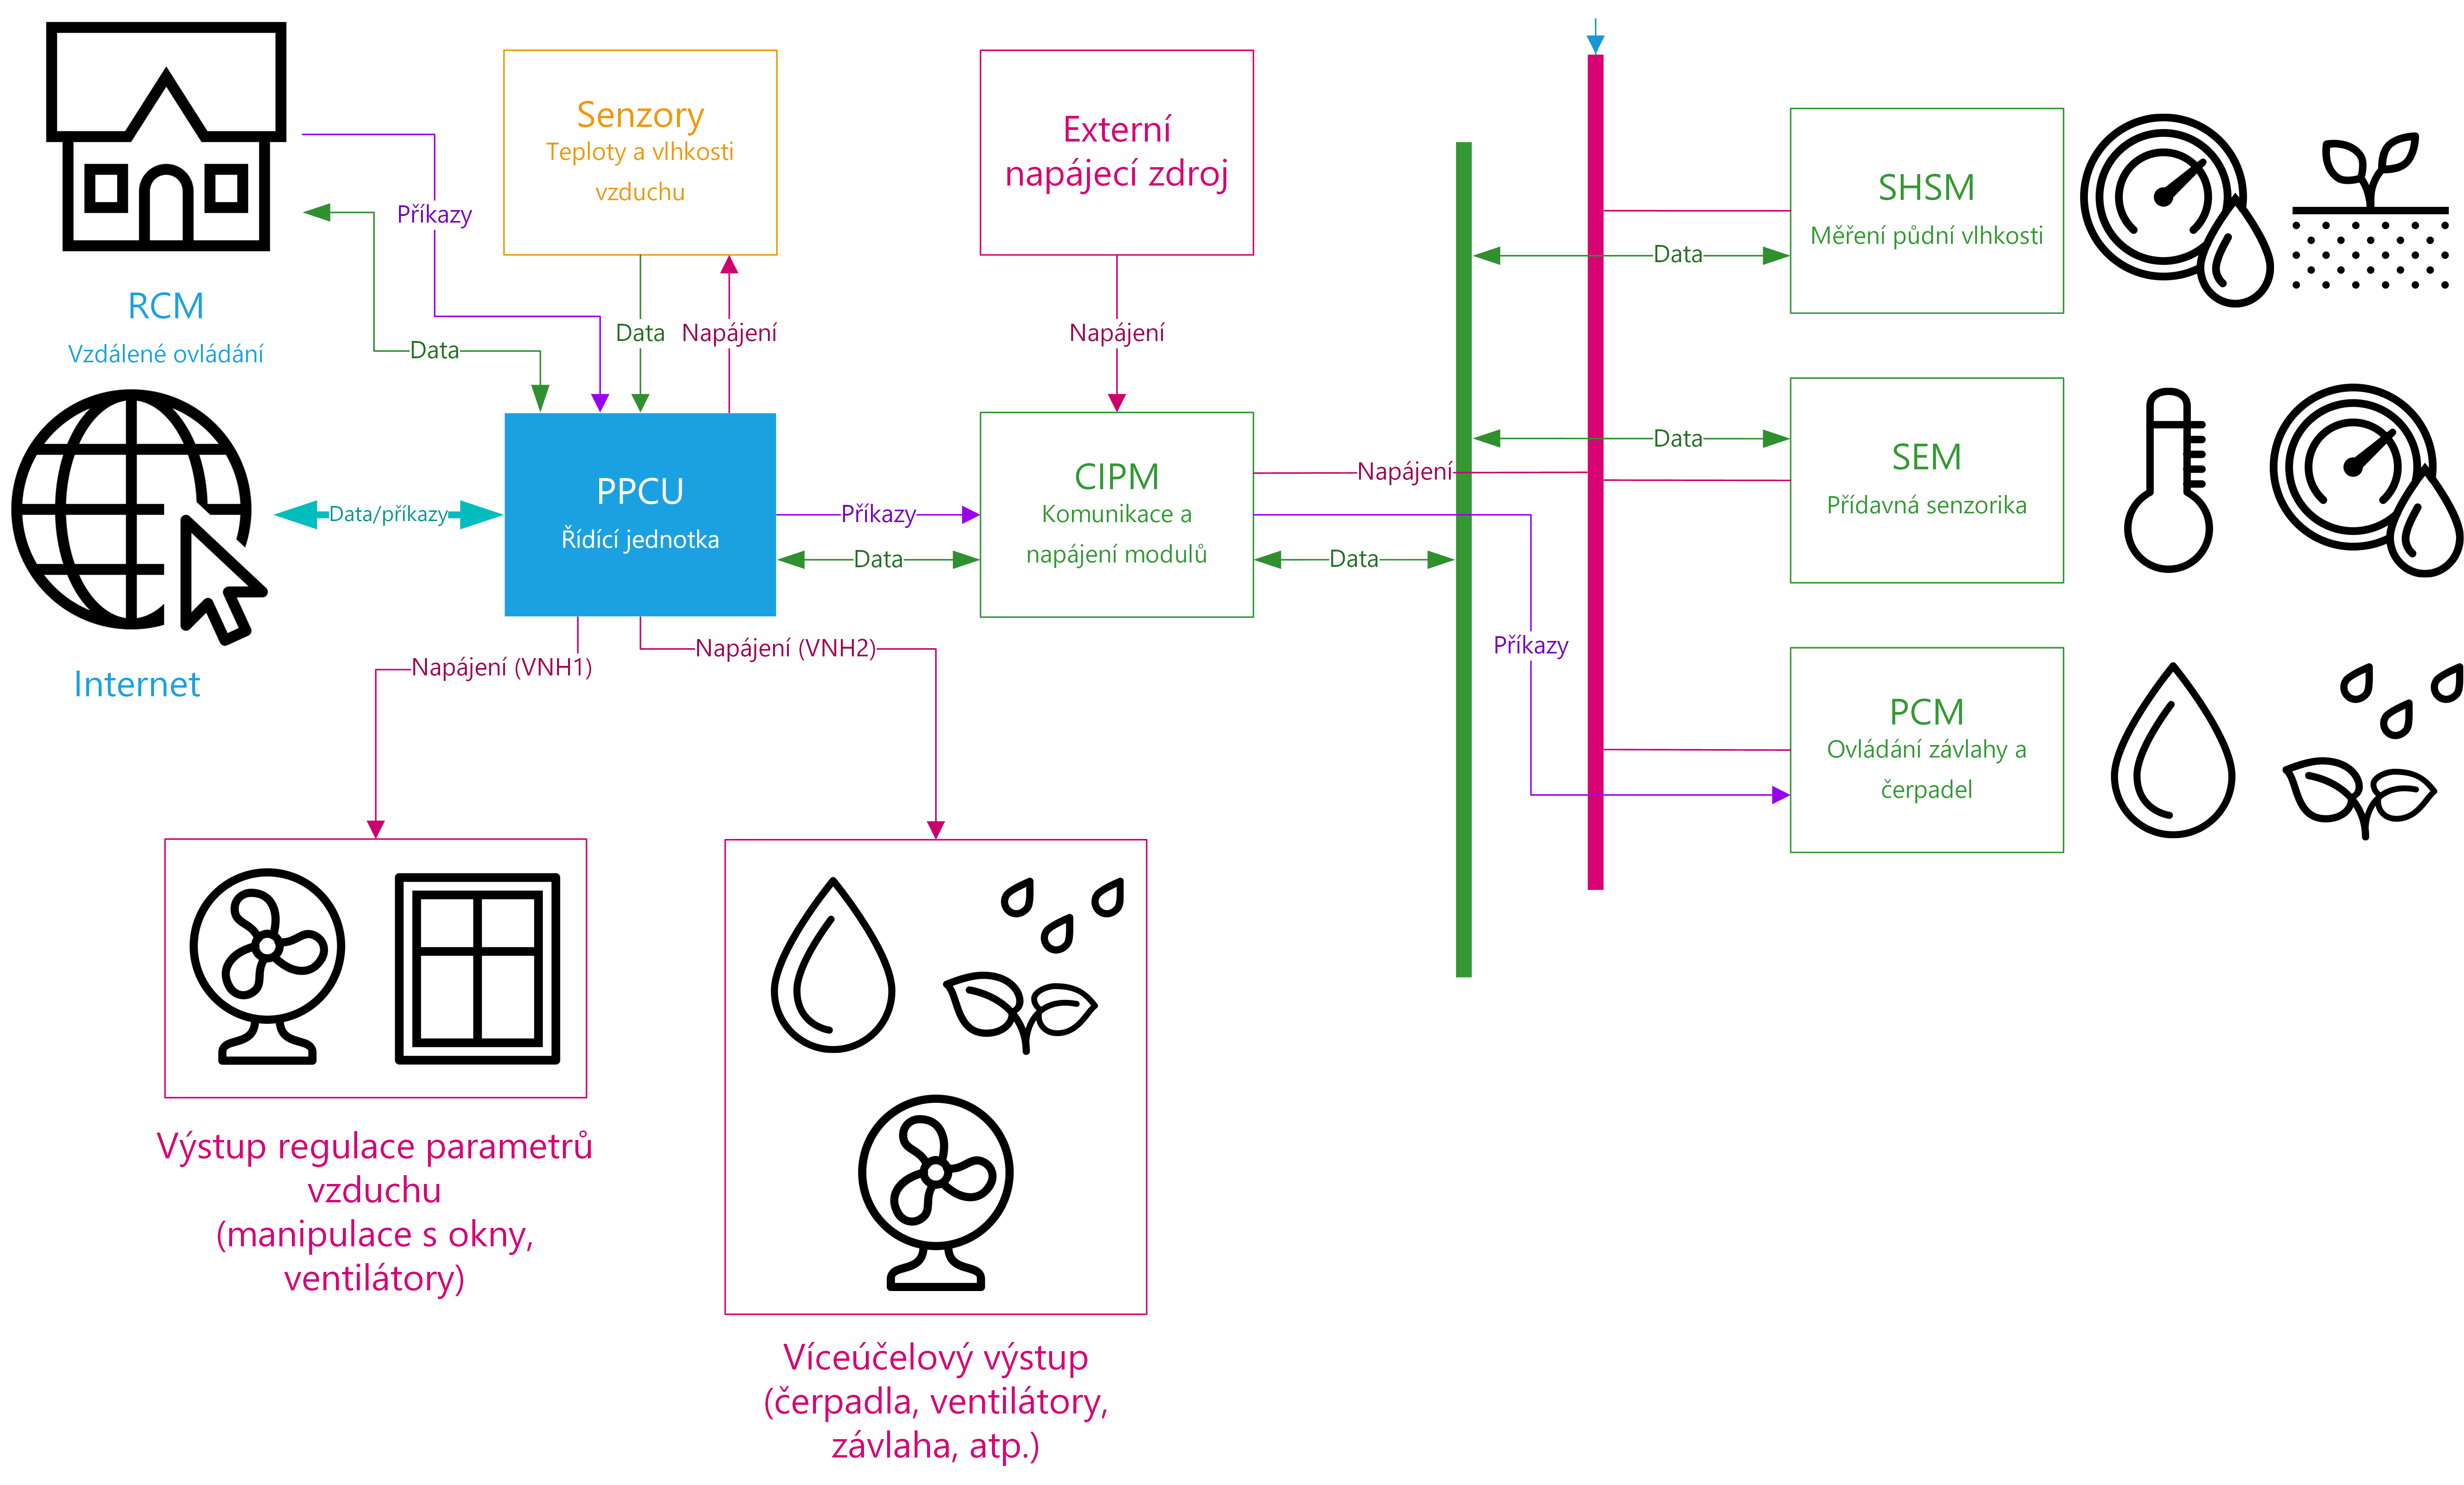
\includegraphics[angle=90,origin=c,scale=0.7]{img/HARDWARE/MODULES.png}
    \caption{Schéma zapojení a~funkce jednotlivých modulů.}
    \label{fig:add-MODULES}
 \end{figure}

\begin{figure}[h]
    \centering
    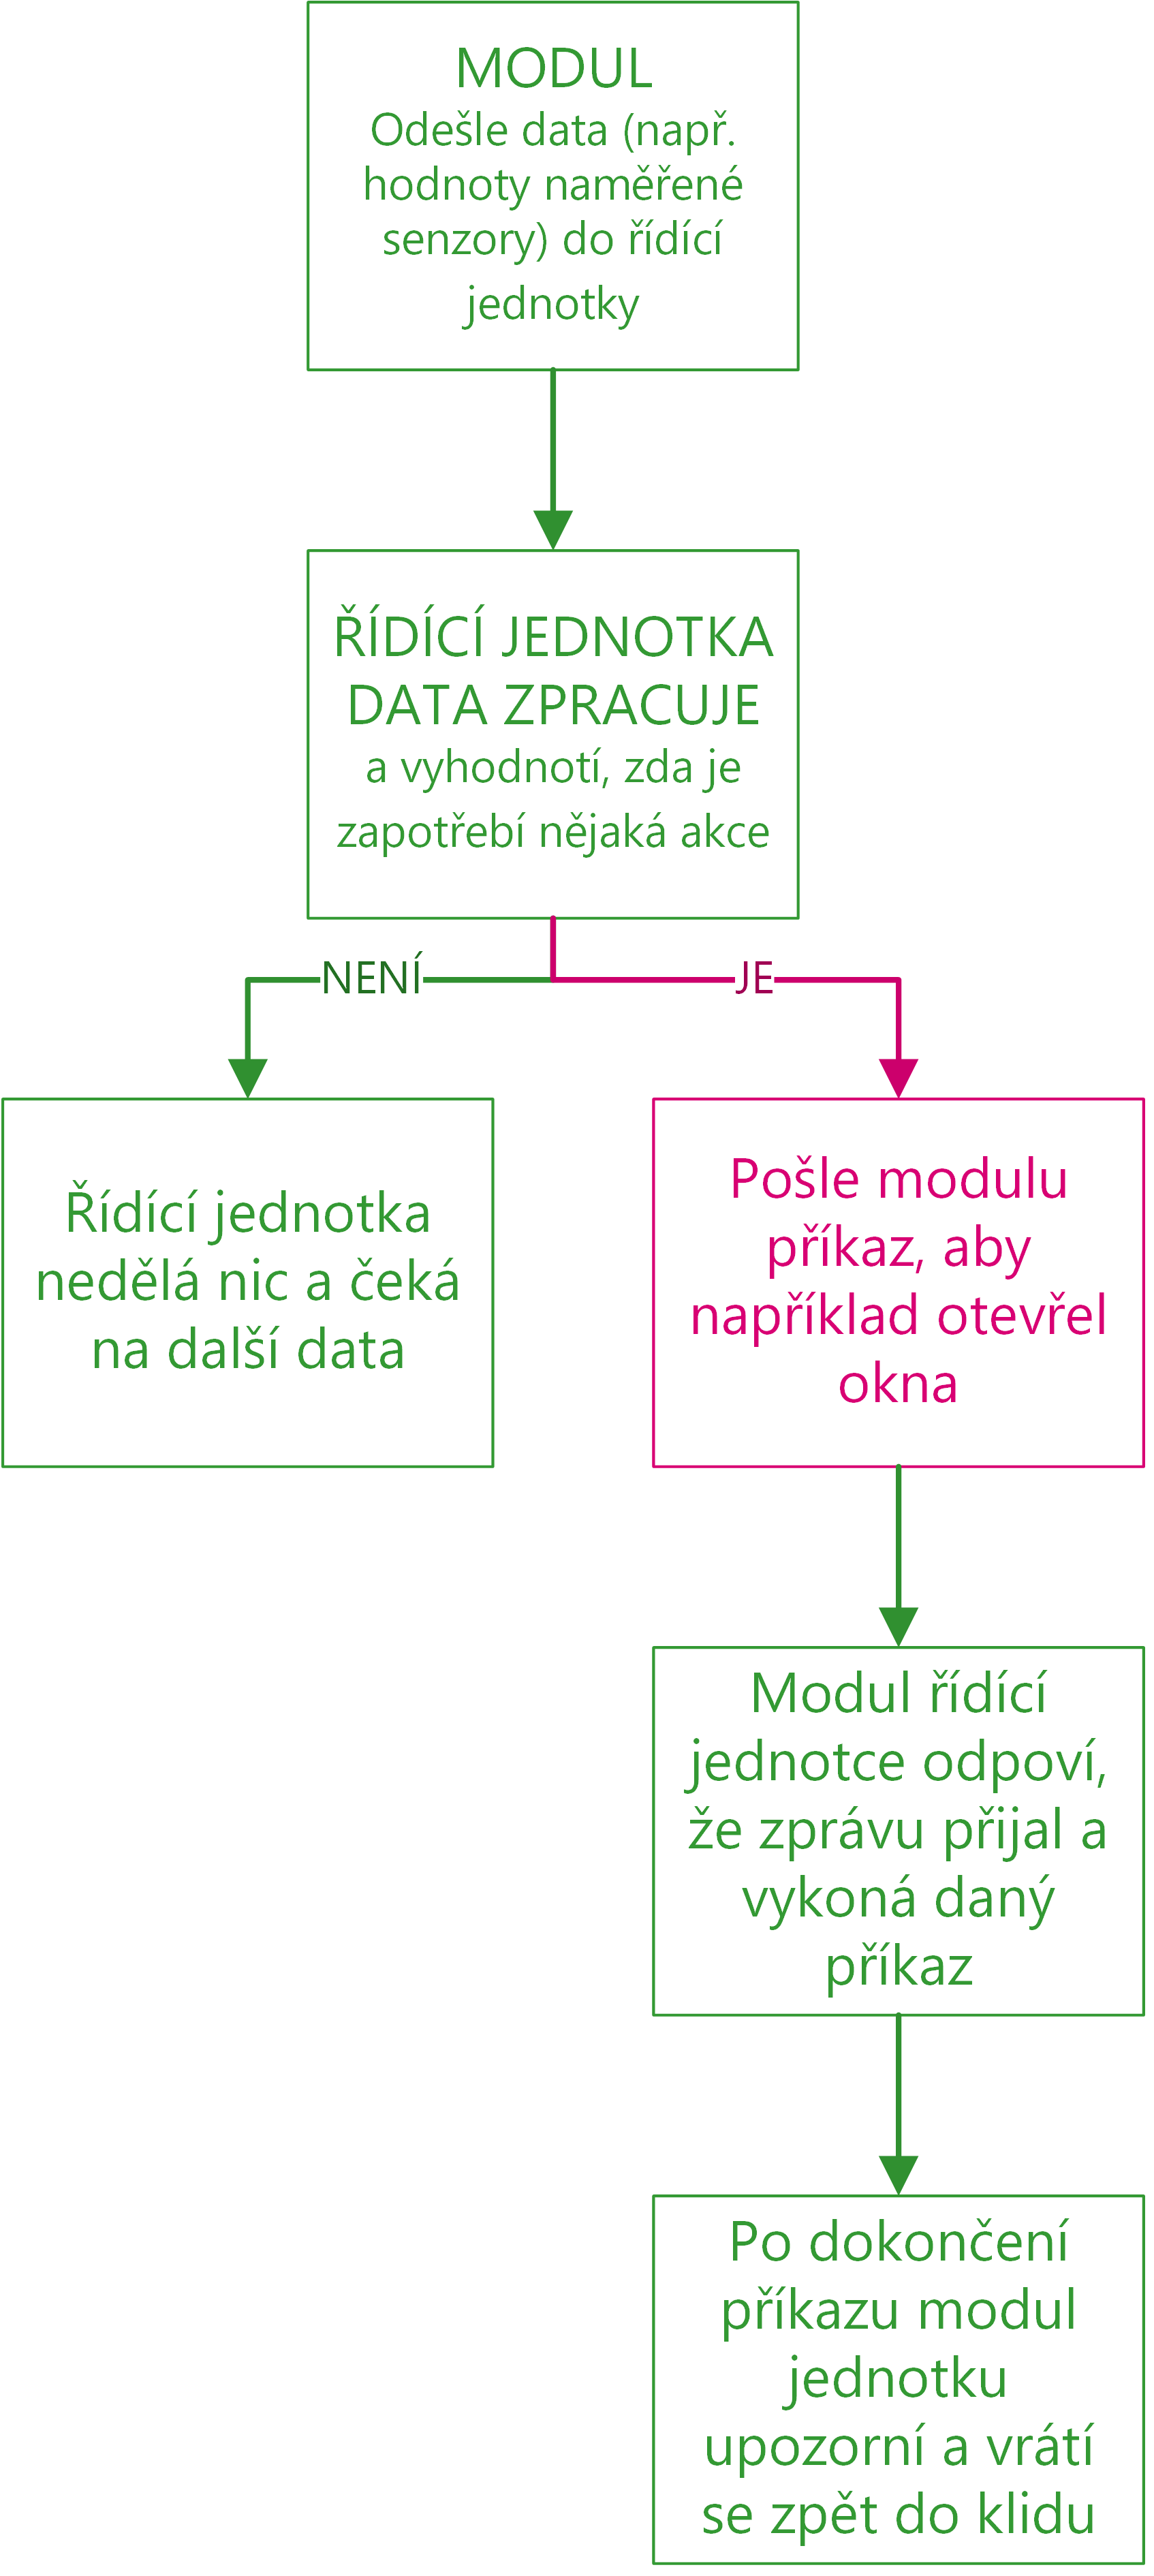
\includegraphics[scale=0.9]{img/SOFTWARE/KOMUNIKACE_MODULU.png}
    \caption{Blokový diagram komunikace řídící jednotky a~přídavného modulu.}
    \label{fig:PPCU-to-MODULE-communication}
\end{figure}

Stejným způsobem lze sázet další obrazové přílohy.
\newpage

\printbibliography[title=Literatura]
\addcontentsline{toc}{chapter}{Literatura}

\listoffigures
\addcontentsline{toc}{section}{Seznam obrázků}

\listoftables
\addcontentsline{toc}{section}{Seznam tabulek}

\end{document}